\afterpage{
    \begin{figure}[t!]
        \centering
        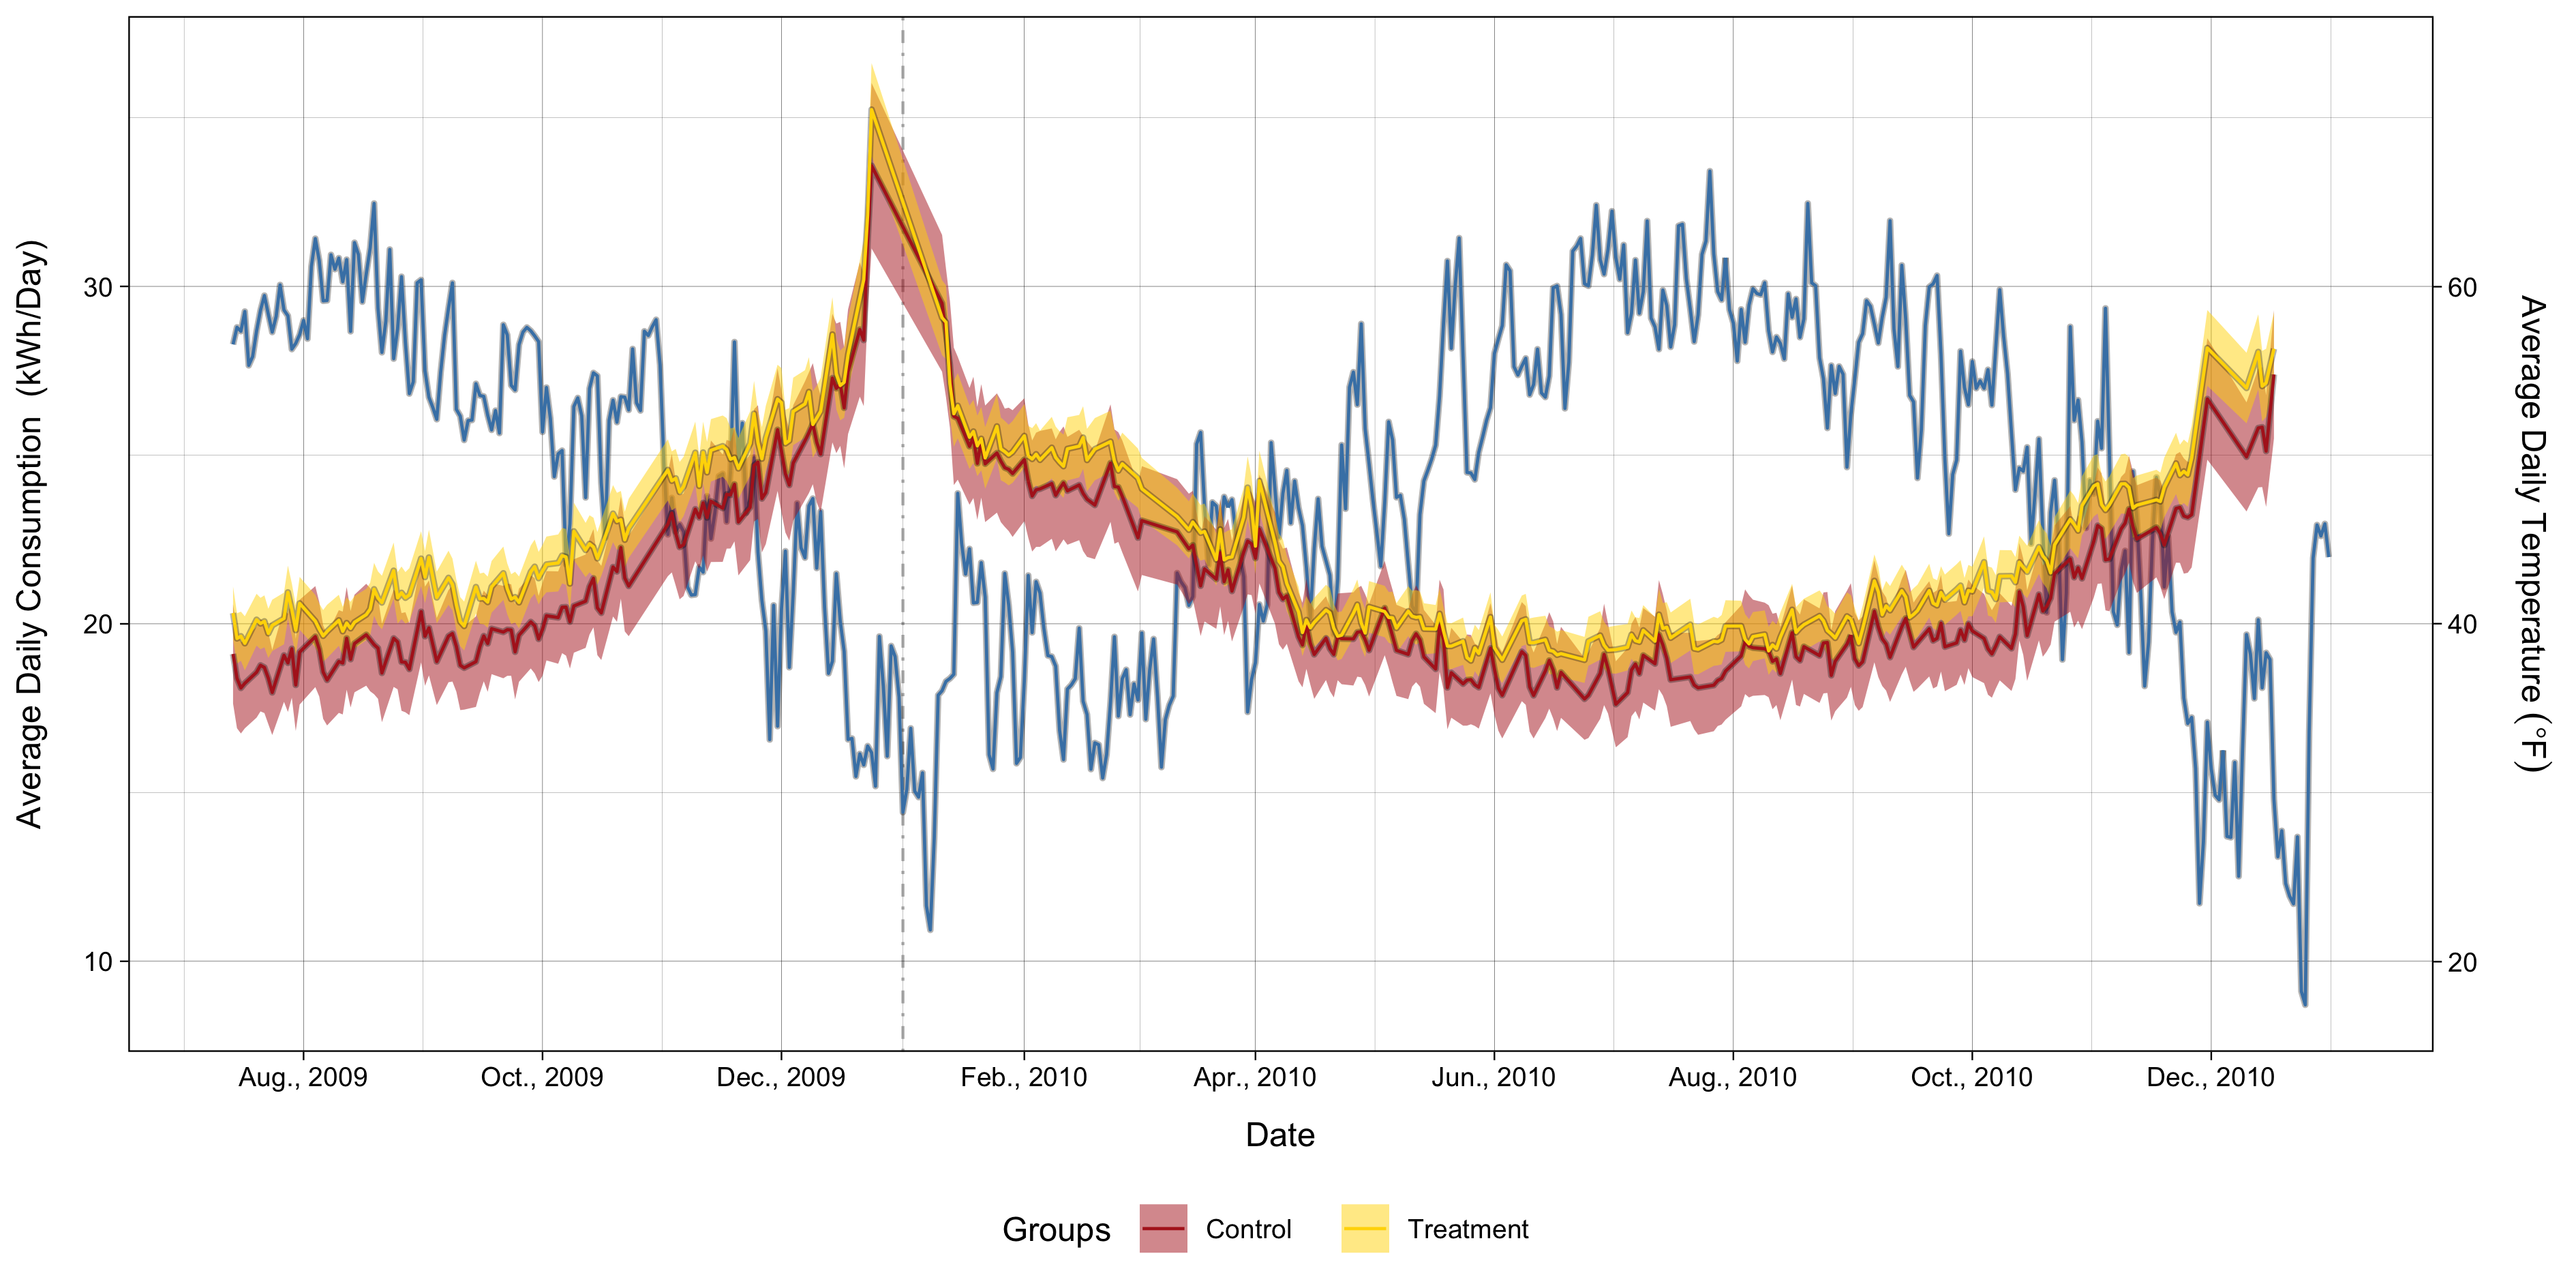
\includegraphics[scale = 0.10]{03_Chapter-2/00A_Figures/Figure_Average-Electricity-Consumption_Average-Daily-Consumption-by-Date.png}
        \caption{Average Daily Electricity Consumption}
        \caption*{
            {\small
            \textit{Note}: The figure depicts, for households that exploit non-electric energy sources for their space and water heating, not only the average daily electricity consumption with 95\% confidence intervals for each group (red and yellow lines) but also the mean daily temperature (blue line). From this figure, it is apparent that household daily electricity consumption is negatively correlated with the average daily temperature. In other words, in Ireland, outdoor temperatures are a crucial driver of within-household electricity consumption.
        }}
        \label{Figure:Average-Daily-Electricity-Consumption}
    \end{figure}
}
Figure \ref{Figure:Average-Daily-Electricity-Consumption} indicates the limitations of focusing on aggregate electricity consumption, as many studies have been doing. The figure clearly shows that aggregate household electricity consumption increases as the weather becomes colder in Ireland. Intuitively, the negative correlation between them can be mainly attributable to for-heating electricity consumption, which strongly depends on outdoor temperatures. It is a fact that aggregate residential electricity consumption also includes another type of electricity consumption: electricity consumption that is irrelevant to temperature variation, such as consumption for lighting. Those two broad categories of electricity consumption could react differently to TOU electricity pricing. Electricity consumption for heating can be transferred to a different time of the day (e.g., from 6 p.m. to 4 p.m. to avoid a higher unit price under the TOU tariff structures). On the other hand, electricity consumption for lighting is time sensitive. Due to the difference in the costs of relocating or changing electricity consumption, it is possible that the two channels of household electricity consumption respond to TOU electricity pricing in different ways. Therefore, using aggregate electricity consumption to examine households' responses to the time-varying price scheme enables me to access only the aggregated response. 

Considering the discussion above, I decompose household electricity consumption into two broad categories---non-temp.-control-driven and temp.-control-driven electricity consumption---and examine how each category of electricity consumption responds to the introduction of the TOU tariff structures. The temperature-control-related electricity consumption here means using electricity to satisfy home heating needs (e.g., to warm up space or water). So, the use of electricity for heating strictly depends on each day's weather conditions, especially temperatures. Naturally, the non-temperature-control-associated electricity consumption makes up the rest. 

I exploit daily Heating Degree Days (HDDs), which imply overall heating needs on a given day, to isolate the temperature-control-driven consumption from aggregate household electricity consumption. Because only aggregate metering data is available from the CER experiment dataset, there is no clue allowing me to classify household electricity consumption into two distinct categories in the dataset. To address this challenge, I presume that the portion of household electricity consumption that fluctuates according to daily HDDs is temperature-control-driven electricity consumption. Therefore, the electricity consumption for temperature-control use is additional consumption that appears only on days with non-zero daily HDDs due to household heating needs.

To break down household responses to the TOU program around the peak rate period, I exploit the following DID-style spline regression model:\footnote{The control group's less percentage changes on freezing days, which are illustrated in Figure (\ref{Figure:Pre-and-Post-Treatment-Household-Average-Daily-Electricity-Consumption}) substantiate the use of the DID-style spline regression model in \ref{Eq:Model-Specification_Breakdown-of-Hourly-Average-Treatment-Effect}.}:
\begin{equation}
\small
\begin{split}
    kWh_{ith} \
    & = \ \beta_{1} HDD_{t} \ + \ \beta_{2} HDD_{t}^{*} \\
    & \hspace{0.7cm} + \ \big( \beta_{3} \ + \ \beta_{4} HDD_{t} \ + \ \beta_{5} HDD_{t}^{*} \big) \mathds{1}[\text{Treatment}]_{i} \\
    & \hspace{0.7cm} + \ \big( \beta_{6} \ + \ \beta_{7} HDD_{t} \ + \ \beta_{8} HDD_{t}^{*} \big) \mathds{1}[\text{Post}]_{t} \\
    & \hspace{0.7cm} + \ \big( \beta_{9} \ + \ \beta_{10} HDD_{t} \ + \ \beta_{11} HDD_{t}^{*} \big) \mathds{1}[\text{Treatment \& Post}]_{it} \ + \ \kappa_{dw} \ + \ \epsilon_{ith} 
\end{split}
\label{Eq:Model-Specification_Breakdown-of-Hourly-Average-Treatment-Effect}
\end{equation}
Like (\ref{Eq:Model-Specification_Hourly-Average-Treatment-Effects}), the dependent variable $kWh_{ith}$ is the electricity consumption by household $i$ on the day $t$ during the hour of the day $h$. In this model, the full set of fixed effects in (\ref{Eq:Model-Specification_Hourly-Average-Treatment-Effects}) has been superseded by two indicator variables---the first indicator variable $\mathbb{1}[\text{Treatment}]_{i}$ has the value of 1 if household $i$ is assigned to the treatment group, and the second indicator variable $\mathbb{1}[\text{Post}]_{t}$ equals 1 when the day $t$ is in the treatment period. Although using the fixed effects as in (\ref{Eq:Model-Specification_Hourly-Average-Treatment-Effects}) does not affect the treatment effects of interests, which is expected given the randomization, replacing them with the indicator variables allows for the interpretation of the average consumption by the treatment group to be more straightforward.\footnote{Added indicator variables instead of various fixed effects also enables an easier graphical summary of the regression results.} The model also includes interaction terms between HDD-relevant terms and those indicator variables. In the econometric model, $HDD_{t}$ means the daily heating degree days on the day $t$. And $HDD_{t}^{*}$, which is required to introduce nonlinearity in HDD-associated response to TOU pricing, is mathematically defined as follows:
\begin{equation}
\small
HDD_{t}^{*} \ = \ (HDD_{t} - Knot) \ \times \ \mathbb{1}[HDD_{t} > Knot],
\end{equation}
where $Knot$ is a reference value at which the slope of the predicted line starts to change. For $Knot$, I utilize the value of ten in the following regression analysis because the median values of daily HDDs in the baseline and treatment periods are ten. The term $\kappa_{dw}$ is day-of-week-by-half-hourly-time-window fixed effects. 

The primary coefficients of interest in (\ref{Eq:Model-Specification_Breakdown-of-Hourly-Average-Treatment-Effect}) are $\beta_{9}$, $\beta_{10}$, and $\beta_{11}$. The three coefficients show how much electricity consumption changes in the households assigned to the treatment group changed after implementing the TOU program compared to those in the control group. To be specific, $\beta_{9}$ demonstrates the change in residential electricity consumption for non-temperature-control use. Both $\beta_{10}$ and $\beta_{11}$ collectively represent the change in the amount of electricity consumed to meet household heating needs at given daily HDDs. 

\afterpage{
    \begin{figure}[t!]
        \centering
        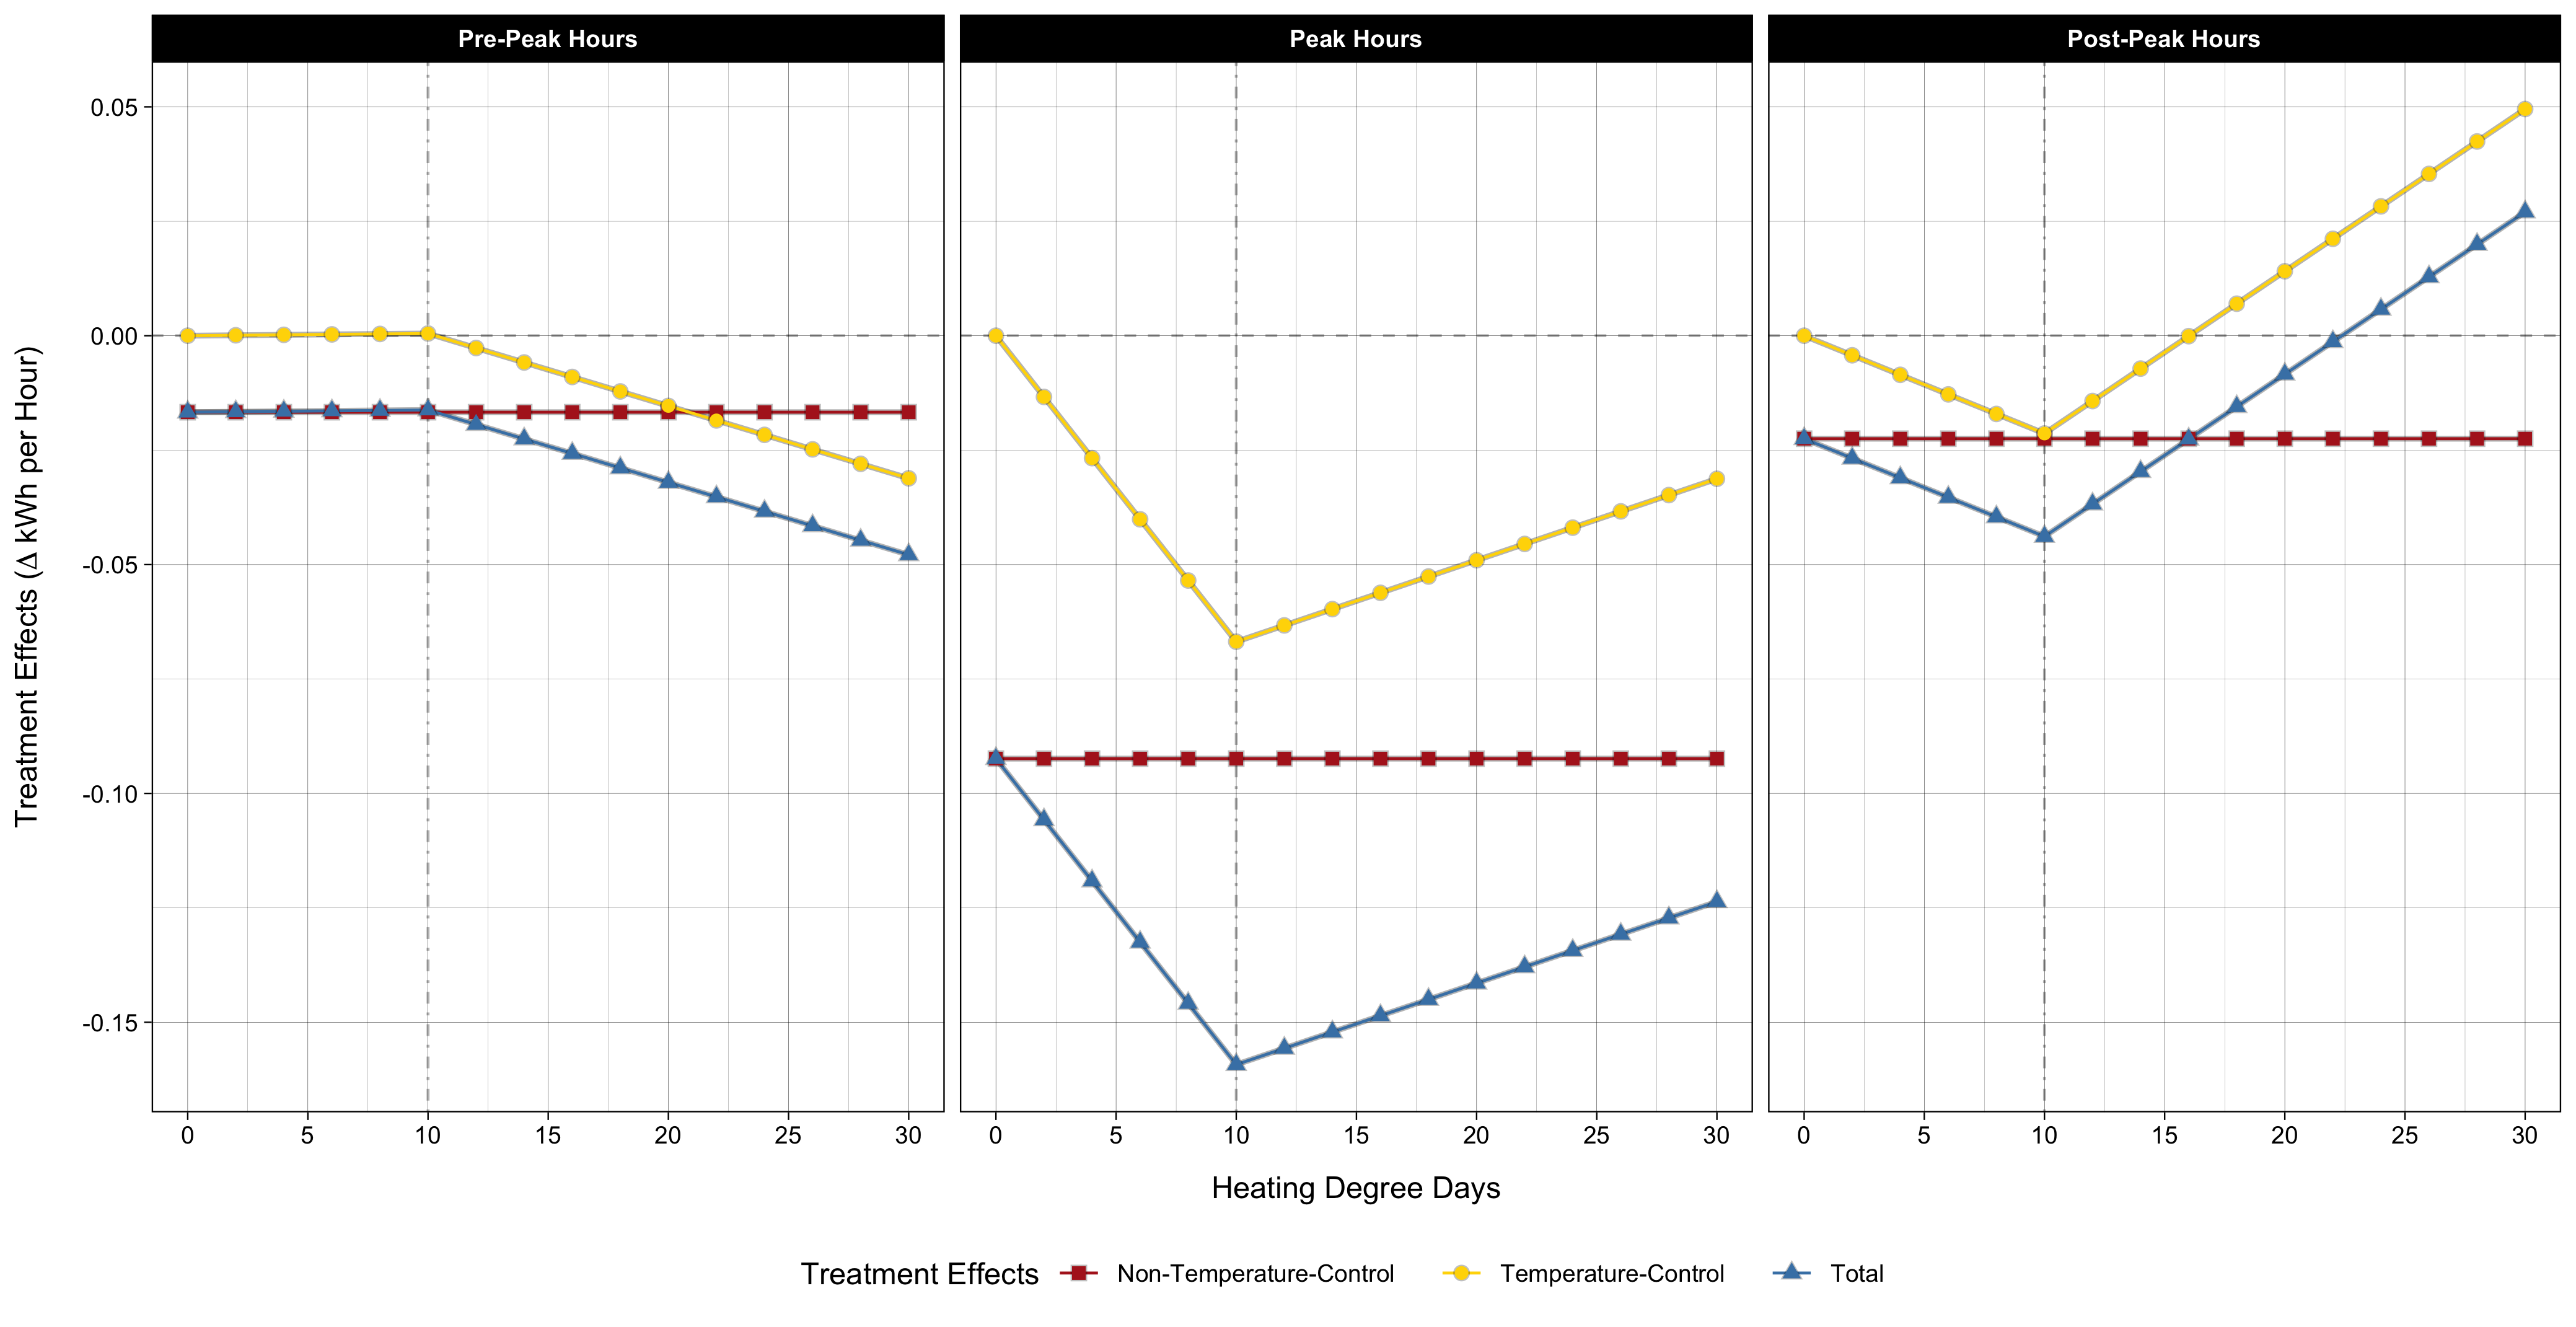
\includegraphics[scale = 0.105]{03_Chapter-2/00A_Figures/Figure_Breakdown-of-Hourly-ATEs_For-Different-Intervals_All_Knot-10.png}
        \caption{Breakdown of Hourly Average Treatment Effects}
        \caption*{
            {\small
            \textit{Note}: This figure is a graphical summary of the regression results. The order of panes corresponds to that of columns. As clearly illustrated, each two-hour interval shows distinct evolving patterns of two broad categories of household electricity consumption. The changes in non-temperature-control-driven household electricity consumption are straight lines because they are independent of outdoor temperature variation. On the other hand, the changes in temperature-control-associated residential electricity consumption are a nonlinear function of daily HDDs.
        }}
        \label{Figure:Breakdown-of-Hourly-ATEs-in-the-Peak-Rate-Period}
    \end{figure}
}
Using the point estimates of the three coefficients of interest, I graphically summarize the predicted change in each of the two channels of electricity consumption in Figure \ref{Figure:Breakdown-of-Hourly-ATEs-in-the-Peak-Rate-Period}. Regarding the change in electricity consumption for non-temperature-control use, the table and figure clearly show that the treated households significantly reduced their consumption when subject to peak-hour prices (i.e., in the peak rate period). Their non-temperature-control-driven electricity consumption also decreased in the pre- and post-peak periods, albeit noisy and relatively smaller in magnitude than the peak-hour changes. 

The change in temperature-control-associated electricity consumption occurred as well in all three two-hour periods, but its evolving pattern over daily HDDs was quite different in each period. Specifically, the impact of TOU pricing on residential electricity consumption for heating was U-shaped in the peak rate period. In contrast, in the hours before and after the peak period, the TOU intervention altered the electricity use for heating only on the coldest days (i.e., only when daily HDDs were sufficiently large). In other words, from the figure, it is evident that the change originating from temperature-control-related electricity consumption was a nonlinear function of daily HDDs in all three periods.

Specification (\ref{Eq:Model-Specification_Breakdown-of-Hourly-Average-Treatment-Effect}) is also utilized to examine, for the peak rate period, the relationship between the degree of a price increase in that period and the change in electricity consumption. On the whole, the reduction stemming from electricity demand for non-temperature-control use tends to be proportional to the size of price growth in peak hours, even though the point estimate for Tariff Group C is an exception. Therefore, the marginally diminishing effects of TOU pricing, discussed in \cite{Peaking-Interest:How-Awareness-Drives-the-Effectiveness-of-Time-of-Use-Electricity-Pricing_Prest_2020}, seem not to be championed by my point estimates. To be specific, while the aggregate electricity consumption during the peak rate period does not sensibly respond to incremental changes in the peak-hour price, the amount of electricity used for non-temperature-control purposes in the peak rate period does respond meaningfully to the marginal changes in the peak price. And the two estimates associated with temperature-control-driven electricity consumption (i.e., $\hat{\beta}_{10}$ and $\hat{\beta}_{11}$) are statistically significant only for the case of the smallest price increase.\footnote{In case of Tariff Group D, only $\hat{\beta}_{11}$ is statistically significant.} 

Altogether, those results imply two interesting points. First, the two distinct types of electricity consumption showed widely different responses to TOU prices in all three periods of two hours. Second, the measured reductions in non-temperature-control-related electricity consumption seem highly sensitive to the magnitude of a price increase in the peak rate period. Inspired by those implications, I formulate the resulting variations in household electricity consumption as a linear function of the magnitude of a rate change in peak-demand hours in the following section.
